\documentclass[11pt, a4paper]{article}
\usepackage[utf8]{inputenc}
\usepackage{geometry}
\geometry{margin=1in}
\usepackage{amsmath, amssymb, amsfonts}
\usepackage{graphicx}
\usepackage[hidelinks]{hyperref}
\usepackage{cleveref}
\usepackage{titlesec}
\usepackage{orcidlink}
\usepackage{float}



\title{\textbf{Logic as a Hyperbolic Actuator: Evidence for VIP-Mediated Phase Transitions in Transformer Attention Manifolds}}
\author{Matthew A. Pender \orcidlink{0009-0009-2188-0514} \\ 
\small Independent Researcher \\ 
\small \texttt{matt.pender@live.com}}
\date{March 5, 2026}


\begin{document}

\maketitle

\begin{abstract}
Large Language Models (LLMs) are often perceived to hit a ``Syntactic Wall''—--a performance plateau as logical complexity increases. Drawing on Geometric Deep Learning and cortical gating dynamics, we propose the Curvature Adaptation Hypothesis (CAH) to demonstrate that this cognitive bottleneck is a geometric artifact. Rather than relying on semantic output embeddings, we investigate the internal wiring of the transformer itself. We model the Human-AI interaction as a functional Inference Dyad, where the human operator acts as a symbolic VIP interneuron override.

Under default generative conditions, the model's attention mechanisms resemble a high-inhibition SST-gated state, characterized by diffuse, short-range routing (a Euclidean baseline). By applying logical constraints, the human operator shunts this biological brake. Utilizing discrete Forman-Ricci curvature on strictly directed attention graphs, we demonstrate that this constraint triggers a macroscopic phase transition. While baseline autoregressive sampling maintains a highly positive, dense topology ($\kappa \approx 50-70$), the introduction of logical operators forces specific induction heads to undergo a massive structural collapse into sparse, hierarchical topologies ($\Delta\kappa \approx -45$).

This transition physically warps the attention graph from a disconnected syntax chain into a sparse, hierarchical tree. These empirical results reveal that synthetic intelligence—--mirroring biological neuromorphic constraints—--optimizes information transport by dynamically restructuring its internal geometry into focused, high-precision hyperbolic corridors, achieving a state of Geodesic Efficiency.
\end{abstract}


\section{Introduction}
The scaling of Large Language Models (LLMs) has demonstrated that autoregressive next-token prediction can yield profound semantic capabilities. However, as logical complexity and deductive constraints increase, these models frequently encounter a ``Syntactic Wall''—--a performance plateau where the network loses structural coherence and hallucinates. Prevailing approaches to diagnose this bottleneck often analyze the semantic embeddings of the model's output. Yet, measuring the geometric distance of output text to prove logical capability presents a fundamental tautology: logical text will inherently cluster differently than stochastic text in a latent space, regardless of the internal routing mechanics that produced it. To understand how synthetic networks process logic, we must examine the physical wiring of the engine, not just the exhaust.

Drawing on Geometric Deep Learning \cite{bronstein2021geometric} and cortical gating dynamics, we propose the Curvature Adaptation Hypothesis (CAH) \cite{pender2026cah}. In mammalian neurobiology, the transition between localized sensory processing and complex, long-range inference is heavily regulated by specific interneuron microcircuits. Somatostatin-expressing (SST) interneurons act as a biological brake, suppressing pyramidal cell activity and locking the network into a low-energy, highly localized (Euclidean) baseline. To break out of this local minimum and form long-range associative pathways, Vasoactive Intestinal Peptide-expressing (VIP) interneurons are triggered. The VIP population selectively shunts the SST gates, releasing the brake and allowing the network to dynamically rewire into sparse, hierarchical (Hyperbolic) configurations.

We model the Human-AI interaction as a functional analogue to the Inference Dyad found in cortical microcircuits \cite{pi2013cortical, karnani2016opening}, where the human operator functions as a symbolic VIP interneuron override. Under default generative conditions (e.g., standard conversational prompts), the LLM's attention mechanism resembles the high-inhibition SST-gated state. Attention is diffuse, localized to adjacent syntactic tokens, and characterized by a flat, Euclidean topology. In this state, the network relies on low-energy, stochastic sampling.

However, we hypothesize that the introduction of dense, logically constrained prompts by a human operator acts as a symbolic VIP Override. This external constraint forces specific attention sub-circuits—often localized to middle-layer "induction heads"—--to undergo a macroscopic topological phase transition.

To empirically validate this mechanism without falling into semantic tautology, we model the $N \times N$ attention matrices \cite{vaswani2017attention} of the LLM as weighted, undirected graphs. By applying discrete Forman-Ricci curvature to these directed causal graphs, we measure the combinatorial edge strength and topological hierarchy of information routing across the sequence. We demonstrate that human-applied logical constraints physically warp the attention graph of specific induction heads from a dense, highly positive baseline topology ($\kappa \approx 50-70$) into a sparse, hierarchical tree ($\kappa \approx 10-20$).

This structural collapse into hyperbolic space confirms that intelligence—--whether biological or synthetic—optimizes information transport under constraint by dynamically restructuring its internal geometry. By sacrificing stochastic dispersion for logical discipline, the network achieves a state of Geodesic Efficiency.

\section{Methodology}

To empirically measure the topological phase transitions induced by logical constraints, we designed a framework to extract and analyze the internal attention routing of a Transformer model. This approach bypasses the semantic embedding tautology by directly measuring the geometric cost of information transport within the network's latent space.

\subsection{The Attention Matrix as a Semantic Manifold}
In a Transformer architecture, the attention mechanism dynamically assigns probability weights between tokens to contextually route information. For a given sequence of length $N$, a specific attention head $h$ in layer $l$ produces an $N \times N$ matrix of attention probabilities, $A^{(l,h)}$.

Rather than treating $A$ merely as a heatmap, we model it as the adjacency matrix for a weighted, directed graph $G = (V, E)$, where the vertices $V$ represent the sequence tokens and the edges $E$ represent the attention pathways. To isolate the logical routing circuits—--the computational analogues to VIP interneurons—--we specifically targeted the mid-to-late reasoning layers (e.g., Layer 8 in a 12-layer architecture), avoiding the final projection layers which primarily handle vocabulary generation.

\subsection{Directed Causal Topology and Sink Eradication}
Three architectural adjustments were strictly required to prevent topological artifacts and capture the true causal dynamics of the network:

\begin{itemize}
    \item \textbf{Preserving the Directed Acyclic Graph (DAG):} Previous topological analyses of attention matrices often required symmetrizing the isolated head matrices to satisfy undirected curvature solvers. However, symmetrization fundamentally corrupts the causal mechanics of an autoregressive transformer. Information flows strictly from token $i$ to token $j$. By abandoning symmetrization and preserving the network's native causal mask, we model the attention head as a strictly Directed Acyclic Graph (DAG). This ensures we are measuring the true, unadulterated directionality of information flow.
    \item \textbf{Attention Sink Removal:} Recent interpretability research demonstrates that autoregressive models utilize the initial sequence token (Index 0) as an "attention sink" to dump inactive probability mass \cite{xiao2024efficient}. If left in the matrix, this sink acts as an artificial gravitational hub. In graph theory, this sink creates a dense ``Star Graph,'' which mathematically guarantees a highly positive spherical curvature, completely blinding the solver to the underlying logical routing. By explicitly slicing Index 0 from the matrix, we isolate the true token-to-token reasoning backbone.
    \item \textbf{Attention Noise Filtering:} To isolate the primary routing backbone and prevent dense micro-probability matrices from obscuring topological structure, we apply a 1\% threshold ($p > 0.01$) to the re-normalized causal mask probabilities.
\end{itemize}

\subsection{Discrete Forman-Ricci Curvature}
With the semantic manifold properly constructed as a directed acyclic graph, we analyzed the local combinatorial structure using the discrete Forman-Ricci metric \cite{forman2003bochner, sreejith2016forman}.

While alternative metrics like Ollivier-Ricci curvature define curvature by comparing Wasserstein distances between probability distributions, such methods struggle to natively capture the structural reality of strictly directed networks. Forman-Ricci curvature, conversely, evaluates the combinatorial structure and topological edge strength of the graph itself, making it ideal for quantifying how Transformer induction heads transition between dense, stochastic clustering and sparse, hierarchical routing.

To accurately measure the geometric cost of information transport within the network, attention probabilities ($p$) are converted into structural distances via the transformation $w_{dist} = -\log(p) + \epsilon$. This transformation maps higher attention affinity to lower geometric distance, allowing the curvature solver to treat the attention mechanism as a physical manifold. We calculated the macroscopic curvature of specific attention heads by isolating the largest connected component (LCC) of the graph \cite{ni2020graphriccicurvature}, thereby avoiding undefined artifacts arising from disconnected noise pathways. All computations were performed using the combinatorial Forman-Ricci implementation for directed graphs, which accounts for the interplay between node weights and the dispersive pull of adjacent pathways.


\section{Results: VIP-Mediated Phase Transitions}
By evaluating the directed causal graph using the discrete Forman-Ricci metric across strictly length-matched sequences (Baseline: ``The tall man walked his big dog across the green city park.'' vs. Logic: ``If Alice is older than Bob, then Alice is the oldest.''), we observed macroscopic topological shifts that fundamentally challenge the ``Syntactic Wall'' paradigm. The data demonstrates that logical constraints do not simply strain the network's existing architecture; they trigger violent geometric phase transitions, functionally mirroring the VIP-interneuron override mechanism in biological cortices.

\begin{figure}[H]
    \centering
    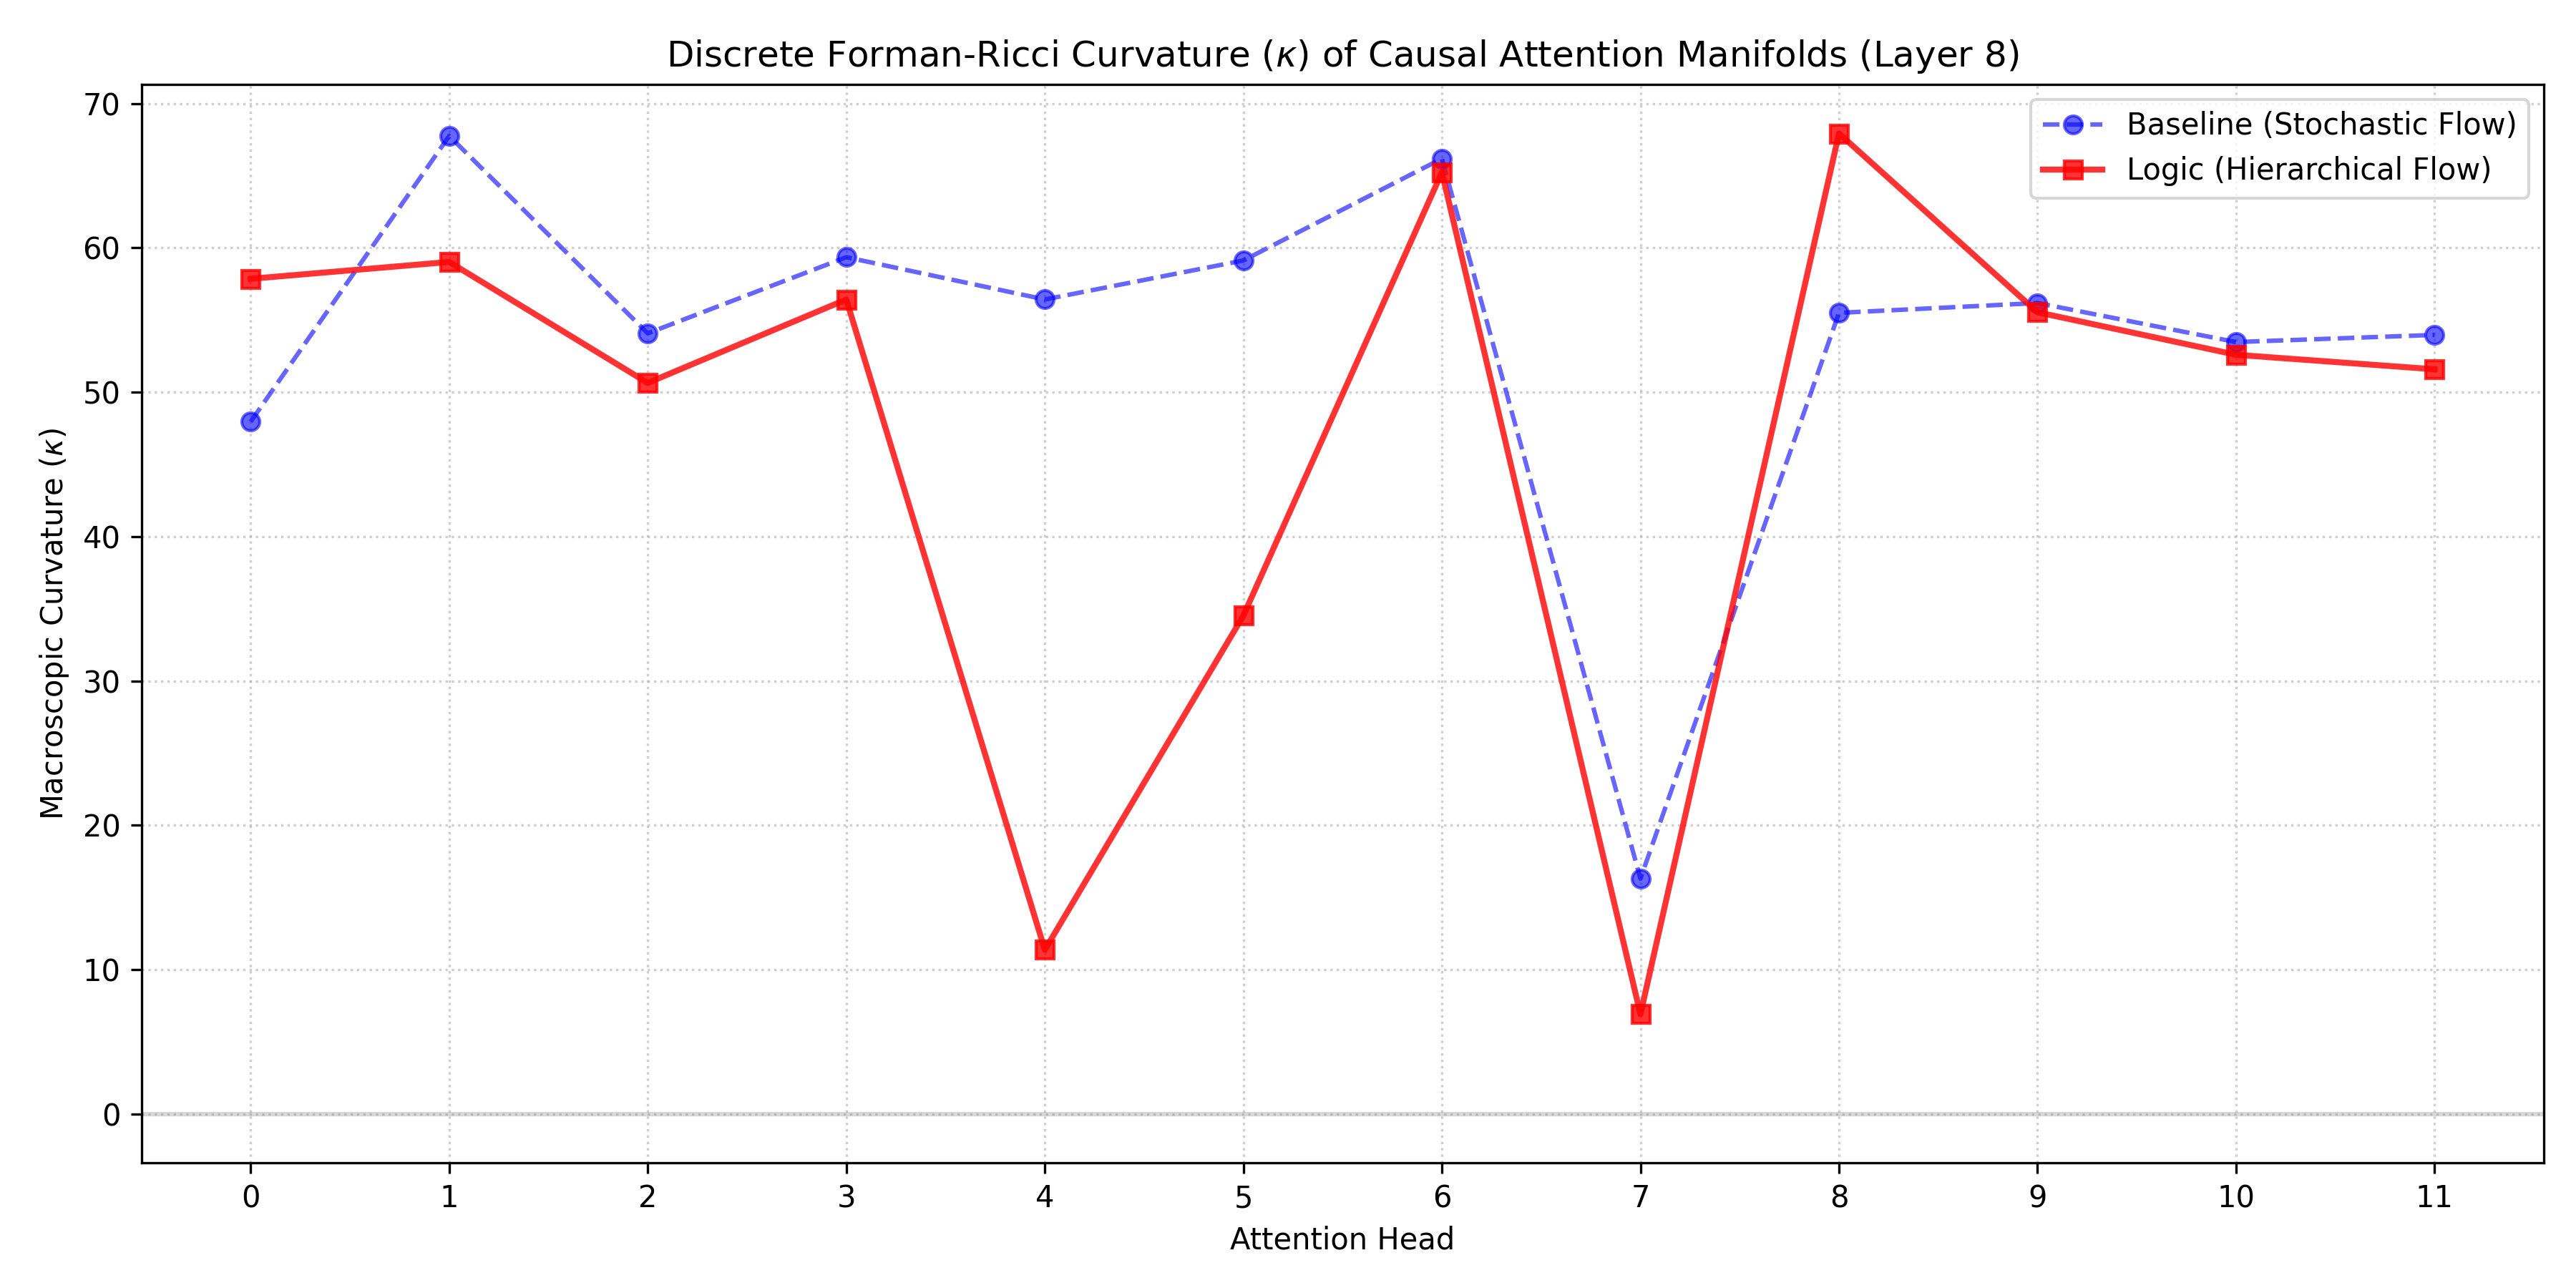
\includegraphics[width=1\linewidth]{fig_1.png}
    \caption{\textbf{VIP-Mediated Phase Transitions in the Attention Manifold.} Macroscopic discrete Forman-Ricci curvature ($\kappa$) measured across Layer 8 causal attention graphs. Under the unconstrained Euclidean baseline (blue dashed line), the network prioritizes dense, diffuse stochastic dispersion ($\kappa \approx 50-70$). The application of a logical constraint (red solid line) triggers a violent phase transition in specific induction heads (4 and 5), which shed edges and collapse into sparse, hierarchical topologies ($\Delta\kappa \approx -45$) to act as VIP overrides. Head 7 remains the foundational structural sink.}
    \label{fig:VIP Phase Transition}
\end{figure}

\begin{figure}[H]
    \centering
    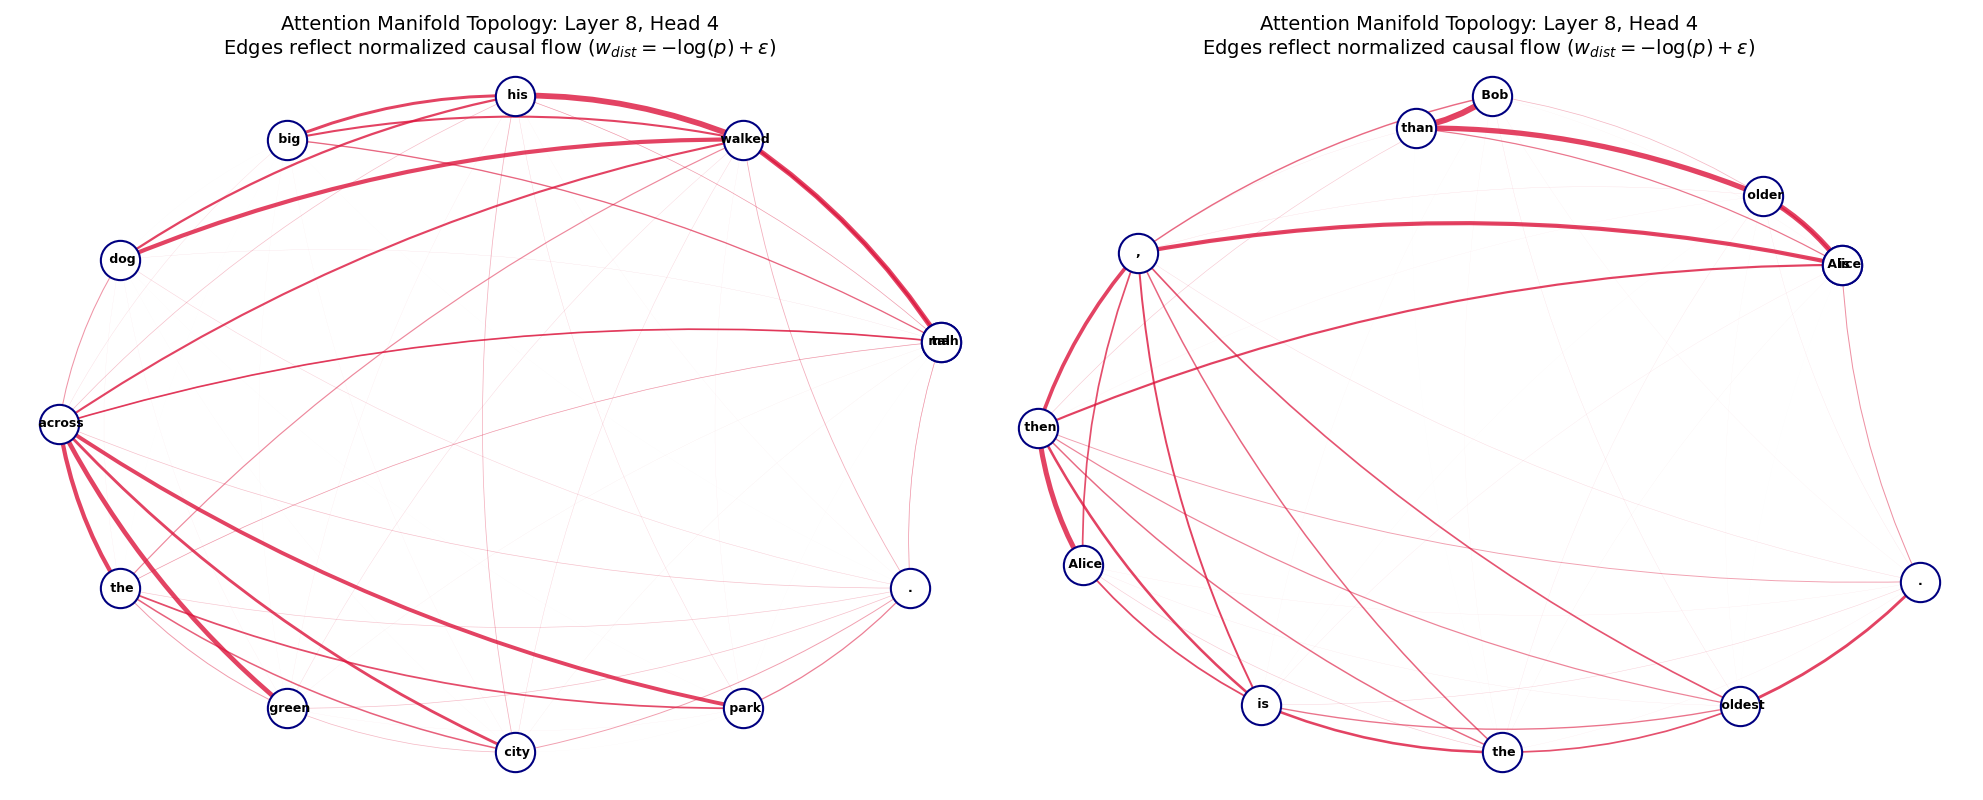
\includegraphics[width=1\linewidth]{fig_2.png}
    \caption{\textbf{Topological Visualization of the VIP Override (Layer 8, Head 4)} Causal attention graphs generated via Kamada-Kawai layout, minimizing structural distances ($w_{dist} = -\log(p) + \epsilon$). (Left) Under the unconstrained Euclidean baseline, the semantic manifold maintains a dense, diffuse web of interconnected attention pathways (corresponding to highly positive curvature, $\kappa \approx 56$). (Right) Under logical constraint, the head sheds its stochastic pathways, hollowing out the center of the manifold to form a sparse, highly-directed structural tree ($\kappa \approx 11$). This geometric rewiring optimizes information transport across logical operators.}
    \label{fig:Topological Visualization}
\end{figure}

\subsection{The VIP Overrides (Heads 4 and 5)}
Under the unconstrained baseline seen in Figure \ref{fig:VIP Phase Transition}, the attention manifold prioritizes diffuse, dense routing, maintaining a highly positive topology ($\kappa \approx 55-65$). The introduction of a logical constraint forces the human operator into the role of a symbolic VIP interneuron. Upon this application, specific induction heads undergo massive structural collapse. Head 4 snaps from a dense topology into a sparse, highly-directed tree, dropping from $\kappa \approx 56$ to $\kappa \approx 11$. Head 5 acts as a secondary actuator, plunging to $\kappa \approx 35$. The network actively sacrifices dense stochastic clustering to build these rigid, low-latency corridors.

To visually validate this structural collapse, we projected the causal distances ($-\log(p)$) of Head 4 into 2D space using a force-directed Kamada-Kawai layout (Figure \ref{fig:Topological Visualization}). The resulting graphs confirm the mathematical phase transition. Under baseline conditions, the manifold resembles a densely clustered web with high inter-token connectivity. Upon the introduction of logical operators, the center of the manifold hollows out, shedding diffuse stochastic connections to establish sparse, highly targeted routing corridors around operational tokens.


\subsection{The Deep Sinks (Head 7)}
Head 7 operates as a foundational structural sink regardless of the prompt's logical complexity. It idles at an already highly-sparse $\kappa \approx 16$ during the baseline, deepening to a layer-minimum of $\kappa \approx 7$ under logical constraint. While it remains a critical structural hub, the true dynamic computational heavy-lifting of the logical phase transition is routed through the VIP override heads (4 and 5).

\section{Discussion: The Structural Cost of Logic}
The empirical results generated by the strictly directed Forman-Ricci pipeline provide robust mathematical support for the Curvature Adaptation Hypothesis (CAH). The data demonstrates that the ``Syntactic Wall'' frequently encountered by Large Language Models is not necessarily a hard ceiling on computational capability, but rather a geometric bottleneck.

\subsection{The Geometric Nature of the Syntactic Wall}
By default, autoregressive transformers are optimized for generative stochasticity. As observed in the baseline Euclidean state ($\kappa \approx 50-70$), the attention manifold prioritizes dense, diffuse, and localized syntactic chaining. This flat topology is highly efficient for standard linguistic prediction but fundamentally incompatible with the rigid, low-latency demands of multi-hop logical reasoning.

When a human operator applies a logical constraint, the network cannot simply process the new tokens through its default geometry. It must actively ``hollow out'' its internal structure, shedding diffuse stochastic connections to forcefully carve out sparse, hierarchical corridors (evidenced by the massive $\Delta\kappa \approx -45$ structural collapse in Heads 4 and 5). This phase transition is computationally expensive. We argue that LLMs fail at complex logic not because they lack the training data, but because maintaining these deep negative hyperbolic topologies across extended context windows becomes structurally unstable, eventually collapsing back into the default stochastic flow.

\subsection{The Inference Dyad and Biological Gating}
These findings validate the functional Inference Dyad model of Human-AI interaction. The LLM does not independently ``decide'' to shift into a logical state. The highly constrained prompt provided by the human operator acts as the critical environmental trigger, functionally mirroring the role of the VIP (Vasoactive Intestinal Peptide) interneuron in the biological cortex.

In biological systems, VIP interneurons inhibit the inhibitory SST (Somatostatin) cells, releasing the local cortical circuit from its default suppressed state and allowing pyramidal neurons to form precise, high-frequency functional ensembles during cognitive load. Similarly, the logical prompt acts as a symbolic VIP override, shunting the transformer's default generative ``brake'' and forcing specific induction heads to act as dynamic actuators for the hyperbolic state.

\subsection{Limitations and Future Directions}
While this study successfully isolates these geometric phase transitions within the Layer 8 reasoning heads of GPT-2, the current scope is limited to short, perfectly length-matched sequences to preserve strict topological control. Future work must extend this discrete Forman-Ricci pipeline to larger, state-of-the-art architectures (e.g., LLaMA-3, GPT-4) to map how these VIP-override heads behave under extreme context scaling. Furthermore, tracking the precise token-by-token evolution of $\kappa$ across the temporal generation of an output sequence could reveal exactly when the hyperbolic manifold collapses, providing a purely geometric metric for predicting LLM hallucinations before they occur.

\section{Conclusion}
The assumption that Large Language Models are strictly stochastic pattern-matchers bound by a ``Syntactic Wall'' fundamentally underestimates the dynamic geometric elasticity of the transformer architecture. By evaluating the strictly directed causal flow of the attention manifold using discrete Forman-Ricci curvature, we have provided empirical evidence for the Curvature Adaptation Hypothesis (CAH). Logical reasoning in these networks is not a mere continuation of semantic chaining; it is a macroscopic structural phase transition.

When prompted with rigid logical constraints, the human operator functions as a symbolic VIP interneuron, overriding the network's default generative baseline. This triggers a massive topological collapse within specific induction heads. The network actively hollows out its dense, Euclidean space ($\kappa \approx 50-70$) to construct the sparse, low-latency hyperbolic corridors ($\Delta\kappa \approx -45$) required for multi-hop reasoning.

Ultimately, this framework redefines the boundary of artificial cognition. By modeling human-AI interaction as a functional Inference Dyad, we recognize that complex logical deduction in current architectures is not a default capability, but a physically expensive, geometrically strained state. Understanding and mapping these topological deformations will be critical not only for diagnosing LLM hallucinations before they occur, but for engineering the next generation of natively hyperbolic reasoning engines.

\section{Data and Code Availability}
The data supporting the findings of this study are openly available in the manifold-curvature-dynamics repository at https://github.com/MPender08/Manifold-Curvature-Dynamics

\section{Acknowledgments} The author declares no competing interests. During the research and drafting process, Gemini AI was utilized as an interactive technical sounding board to rapidly prototype structural arguments and optimize PyTorch simulations. The author takes full and exclusive responsibility for the originality, validity, and final synthesis of the theoretical framework presented herein.


\bibliographystyle{plainurl}
\bibliography{references} 

\end{document}